%%%%%%%%%%%%
%%%%%%%%%%%%
\begin{figure}
\centering
%%%%%%%%%%%%
\pgfdeclarelayer{background}
\pgfsetlayers{background,main}
%%%%%%%%%%%%
%%%%%%%%%%%%

\begin{subfigure}[t]{.22\textwidth}
	\centering
	\fbox{
\includegraphics[width=\textwidth]{fig/mixing/example_t0.png}}
    	\caption{$t=0$}
	\label{fig:mixing_example_0}
\end{subfigure} \quad
\begin{subfigure}[t]{.22\textwidth}
	\centering
	\fbox{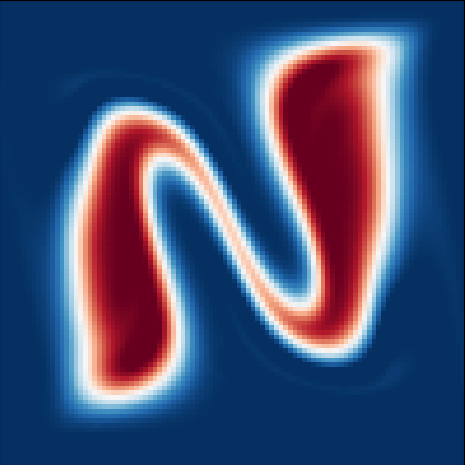
\includegraphics[width=\textwidth]{fig/mixing/example_t10.png}}
    	\caption{$t=10$}
	\label{fig:mixing_example_10}
\end{subfigure} \quad
\begin{subfigure}[t]{.22\textwidth}
	\centering
	\fbox{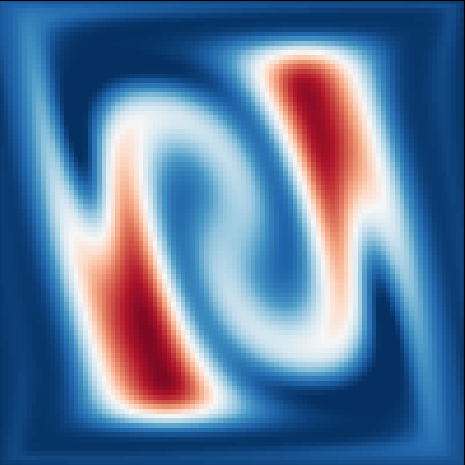
\includegraphics[width=\textwidth]{fig/mixing/example_t30.png}}
    	\caption{$t=30$}
	\label{fig:mixing_example_30}
\end{subfigure} \quad
\begin{subfigure}[t]{.22\textwidth}
	\centering
	\fbox{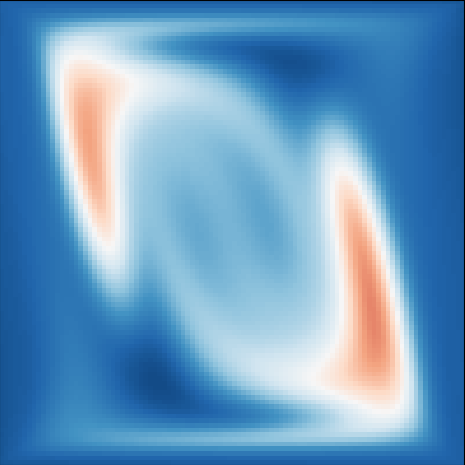
\includegraphics[width=\textwidth]{fig/mixing/example_t60.png}}
    	\caption{$t=60$}
	\label{fig:mixing_example_60}
\end{subfigure}

%%%%%%%%%%%%
\caption{\textbf{Evolution of the concentration in time} with constant boundary conditions $(v_l, v_r, u_b, u_t) = (0, 0, 1.0, -1.0)$.}
\label{fig:mixing_example}
\end{figure} 
%%%%%%%%%%%%
%%%%%%%%%%%%